\documentclass[11pt]{article}
\usepackage{enumitem}
\usepackage{listings}
\usepackage{tikz}
\usepackage{url}
%\usepackage{algorithm2e}
\usetikzlibrary{arrows,automata,shapes}
\tikzstyle{block} = [rectangle, draw, fill=blue!20, 
    text width=5em, text centered, rounded corners, minimum height=2em]
\tikzstyle{bt} = [rectangle, draw, fill=blue!20, 
    text width=4em, text centered, rounded corners, minimum height=2em]

\lstset{ %
language=Java,
basicstyle=\ttfamily,commentstyle=\scriptsize\itshape,showstringspaces=false,breaklines=true,numbers=left}

\newtheorem{defn}{Definition}
\newtheorem{crit}{Criterion}

\newcommand{\handout}[5]{
  \noindent
  \begin{center}
  \framebox{
    \vbox{
      \hbox to 5.78in { {\bf Software Testing, Quality Assurance and Maintenance } \hfill #2 }
      \vspace{4mm}
      \hbox to 5.78in { {\Large \hfill #5  \hfill} }
      \vspace{2mm}
      \hbox to 5.78in { {\em #3 \hfill #4} }
    }
  }
  \end{center}
  \vspace*{4mm}
}

\newcommand{\lecture}[4]{\handout{#1}{#2}{#3}{#4}{Lecture #1}}
\topmargin 0pt
\advance \topmargin by -\headheight
\advance \topmargin by -\headsep
\textheight 8.9in
\oddsidemargin 0pt
\evensidemargin \oddsidemargin
\marginparwidth 0.5in
\textwidth 6.5in

\parindent 0in
\parskip 1.5ex
%\renewcommand{\baselinestretch}{1.25}

\usepackage{fontspec}
\setmonofont{Cousine}[Scale=MatchLowercase]

\begin{document}

\lecture{7 (worksheet) --- January 21, 2019}{Winter 2019}{Patrick Lam}{version 1}

\section*{Active Learning Exercise}
Where are the basic blocks?
\begin{center}
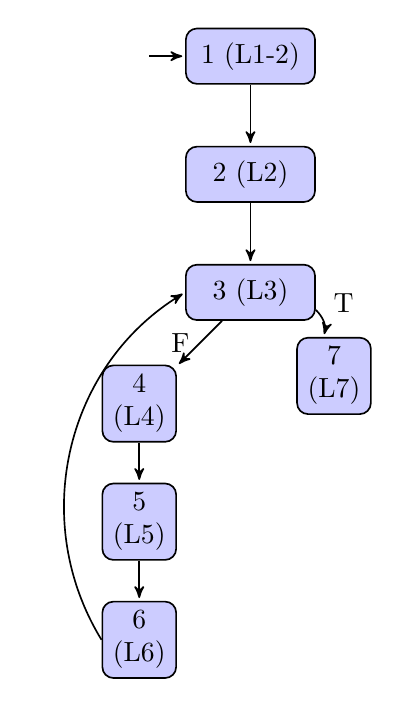
\begin{tikzpicture}[->,>=stealth',shorten >=1pt,auto,node distance=1.5cm,
                    semithick,initial text=]

  \node[initial,bt]   (1)                     {1 (L1-2)};
  \node[bt]           (2) [below of=1]        {2 (L2)};
  \node[bt]           (3) [below of=2] {3 (L3)};
  \node[bt, text width=2em]           (4) [below left of=3,xshift=-1em,yshift=-1em] {4 (L4)};
  \node[bt, text width=2em]           (5) [below of=4,yshift=0em] {5 (L5)};
  \node[bt, text width=2em]           (6) [below of=5,yshift=0em] {6 (L6)};
  \node[bt, text width=2em]           (7) [below right of=3] {7 (L7)};

  \path (1) edge node {} (2)
        (2) edge node {} (3)
        (3) edge node[left] {F} (4)
            edge [bend left] node {T} (7)
        (4) edge node {} (5)
        (5) edge node {} (6)
        (6.west) edge [bend left=45] node {} (3.west);
\end{tikzpicture}
\end{center}

{\bf if statements:} What's the control flow graph fragment?

{
  \begin{tabular}{ll}
  \begin{minipage}{.5\textwidth} \begin{lstlisting}
if (z < 17)
  print (x);
else
  print (y);
    \end{lstlisting}
  \end{minipage}
  \begin{minipage}{.5\textwidth} 
\begin{lstlisting}
if (z < 17)
  print(x);
\end{lstlisting}
\end{minipage}
\end{tabular}
}

Short-circuit {\tt if} evaluation is more complicated and is why Jacoco can
sometimes give mysterious branch coverage results.

\begin{lstlisting}
if (z < 17 || q > 8)
  print (x);
else
  print (y);
\end{lstlisting}

\newpage

{\bf while statements:}

\begin{lstlisting}
x = 0; y = 20;
while (x < y) {
  x ++; y --;
}
\end{lstlisting}

{\bf for statements:} 

\begin{lstlisting}
for (int i = 0; i < 57; i++) {
  if (i % 3 == 0) {
    print (i);
  }
}
\end{lstlisting}

{\bf Enhanced for loops:} 
\begin{lstlisting}
for (Widget w : widgetList) {
  decorate(w);
}
\end{lstlisting}


{\bf case / switch statements:} 

\begin{lstlisting}
switch (n) {
  case `I': ...; break;
  case `J': ...; // fall thru
  case `K': ...; break;
}
\end{lstlisting}

{\bf Larger examples:}
\begin{lstlisting}[basicstyle=\scriptsize\ttfamily]
  /** Binary search for target in sorted subarray a[low..high] */
  int binary_search(int[] a, int low, int high, int target) {
    while (low <= high) {
      int middle = low + (high-low)/2;
      if (target < a[middle)
        high = middle - 1;
      else if (target > a[middle])
        low = middle + 1;
      else
        return middle;
    }
    return -1; /* not found in a[low..high] */
  }
\end{lstlisting}

\begin{lstlisting}[basicstyle=\scriptsize\ttfamily]
/* effects: if x==null, throw NullPointerException
            otherwise, return number of elements in x that are odd, positive or both. */
int oddOrPos(int[] x) {
  int count = 0;
  for (int i = 0; i < x.length; i++) {
    if (x[i]%2 == 1 || x[i] > 0) {
      count++;
    }
  }
  return count;
}

// example test case: input: x=[-3, -2, 0, 1, 4]; output: 3  
\end{lstlisting}

\newpage
Finally, we have a really poorly-designed API (I'd give it a D at most,
maybe an F) because it's impossible to succinctly describe what it
does. {\bf Do not design functions with interfaces like this.} But we
can still draw a CFG, no matter how bad the code is.
\begin{lstlisting}[basicstyle=\scriptsize\ttfamily]
  /** Returns the mean of the first maxSize numbers in the array,
      if they are between min and max. Otherwise, skip the numbers. */
  double computeMean(int[] value, int maxSize, int min, int max) {
    int i, ti, tv, sum;

    i = 0; ti = 0; tv = 0; sum = 0;
    while (ti < maxSize) {
      ti++;
      if (value[i] >= min && value[i] <= max) {
        tv++;
        sum += value[i];
      }
      i++;
    }
    if (tv > 0)
      return (double)sum/tv;
    else
      throw new IllegalArgumentException();
  }
\end{lstlisting}



\end{document}
